\documentclass[a4paper,twoside]{article}
%DIF LATEXDIFF DIFFERENCE FILE
%DIF DEL Submitted manuscript
%DIF ADD Camera-ready revision
\usepackage[T1]{fontenc}
\usepackage{graphicx}
\usepackage{calc}
\usepackage{amssymb}
\usepackage{amsmath}
\usepackage{pslatex}
\usepackage{apalike}
\usepackage{booktabs}
\usepackage{algorithm2e}
\usepackage[bottom]{footmisc}
\usepackage[hidelinks,breaklinks]{hyperref}
\usepackage{SCITEPRESS}
%DIF < \hypersetup{pdftitle={Linking Candidate Coverage to Decision Quality: A Framework for LLM Planning Evaluation},pdfauthor={},pdfsubject={Anonymous position paper},pdfkeywords={LLM Planning, Semantic Validation, Evaluation},pdfcreator={LaTeX}}
%DIF -------
\hypersetup{pdftitle={Linking Candidate Coverage to Decision Quality: A Framework for LLM Planning Evaluation},pdfauthor={Alexander V. Mantzaris and James H. Korris},pdfsubject={Revised ICAART 2027 position paper},pdfkeywords={LLM Planning, Semantic Validation, Evaluation},pdfcreator={LaTeX}} %DIF > 
%DIF PREAMBLE EXTENSION ADDED BY LATEXDIFF
%DIF UNDERLINE PREAMBLE %DIF PREAMBLE
\RequirePackage[normalem]{ulem} %DIF PREAMBLE
\RequirePackage{color}\definecolor{RED}{rgb}{1,0,0}\definecolor{BLUE}{rgb}{0,0,1} %DIF PREAMBLE
\providecommand{\DIFaddtex}[1]{{\protect\color{blue}\uwave{#1}}} %DIF PREAMBLE
\providecommand{\DIFdeltex}[1]{{\protect\color{red}\sout{#1}}}                      %DIF PREAMBLE
%DIF SAFE PREAMBLE %DIF PREAMBLE
\providecommand{\DIFaddbegin}{} %DIF PREAMBLE
\providecommand{\DIFaddend}{} %DIF PREAMBLE
\providecommand{\DIFdelbegin}{} %DIF PREAMBLE
\providecommand{\DIFdelend}{} %DIF PREAMBLE
\providecommand{\DIFmodbegin}{} %DIF PREAMBLE
\providecommand{\DIFmodend}{} %DIF PREAMBLE
%DIF FLOATSAFE PREAMBLE %DIF PREAMBLE
\providecommand{\DIFaddFL}[1]{\DIFadd{#1}} %DIF PREAMBLE
\providecommand{\DIFdelFL}[1]{\DIFdel{#1}} %DIF PREAMBLE
\providecommand{\DIFaddbeginFL}{} %DIF PREAMBLE
\providecommand{\DIFaddendFL}{} %DIF PREAMBLE
\providecommand{\DIFdelbeginFL}{} %DIF PREAMBLE
\providecommand{\DIFdelendFL}{} %DIF PREAMBLE
%DIF HYPERREF PREAMBLE %DIF PREAMBLE
\providecommand{\DIFadd}[1]{\texorpdfstring{\DIFaddtex{#1}}{#1}} %DIF PREAMBLE
\providecommand{\DIFdel}[1]{\texorpdfstring{\DIFdeltex{#1}}{}} %DIF PREAMBLE
\newcommand{\DIFscaledelfig}{0.5}
%DIF HIGHLIGHTGRAPHICS PREAMBLE %DIF PREAMBLE
\RequirePackage{settobox} %DIF PREAMBLE
\RequirePackage{letltxmacro} %DIF PREAMBLE
\newsavebox{\DIFdelgraphicsbox} %DIF PREAMBLE
\newlength{\DIFdelgraphicswidth} %DIF PREAMBLE
\newlength{\DIFdelgraphicsheight} %DIF PREAMBLE
% store original definition of \includegraphics %DIF PREAMBLE
\LetLtxMacro{\DIFOincludegraphics}{\includegraphics} %DIF PREAMBLE
\newcommand{\DIFaddincludegraphics}[2][]{{\color{blue}\fbox{\DIFOincludegraphics[#1]{#2}}}} %DIF PREAMBLE
\newcommand{\DIFdelincludegraphics}[2][]{% %DIF PREAMBLE
\sbox{\DIFdelgraphicsbox}{\DIFOincludegraphics[#1]{#2}}% %DIF PREAMBLE
\settoboxwidth{\DIFdelgraphicswidth}{\DIFdelgraphicsbox} %DIF PREAMBLE
\settoboxtotalheight{\DIFdelgraphicsheight}{\DIFdelgraphicsbox} %DIF PREAMBLE
\scalebox{\DIFscaledelfig}{% %DIF PREAMBLE
\parbox[b]{\DIFdelgraphicswidth}{\usebox{\DIFdelgraphicsbox}\\[-\baselineskip] \rule{\DIFdelgraphicswidth}{0em}}\llap{\resizebox{\DIFdelgraphicswidth}{\DIFdelgraphicsheight}{% %DIF PREAMBLE
\setlength{\unitlength}{\DIFdelgraphicswidth}% %DIF PREAMBLE
\begin{picture}(1,1)% %DIF PREAMBLE
\thicklines\linethickness{2pt} %DIF PREAMBLE
{\color[rgb]{1,0,0}\put(0,0){\framebox(1,1){}}}% %DIF PREAMBLE
{\color[rgb]{1,0,0}\put(0,0){\line( 1,1){1}}}% %DIF PREAMBLE
{\color[rgb]{1,0,0}\put(0,1){\line(1,-1){1}}}% %DIF PREAMBLE
\end{picture}% %DIF PREAMBLE
}\hspace*{3pt}}} %DIF PREAMBLE
} %DIF PREAMBLE
\LetLtxMacro{\DIFOaddbegin}{\DIFaddbegin} %DIF PREAMBLE
\LetLtxMacro{\DIFOaddend}{\DIFaddend} %DIF PREAMBLE
\LetLtxMacro{\DIFOdelbegin}{\DIFdelbegin} %DIF PREAMBLE
\LetLtxMacro{\DIFOdelend}{\DIFdelend} %DIF PREAMBLE
\DeclareRobustCommand{\DIFaddbegin}{\DIFOaddbegin \let\includegraphics\DIFaddincludegraphics} %DIF PREAMBLE
\DeclareRobustCommand{\DIFaddend}{\DIFOaddend \let\includegraphics\DIFOincludegraphics} %DIF PREAMBLE
\DeclareRobustCommand{\DIFdelbegin}{\DIFOdelbegin \let\includegraphics\DIFdelincludegraphics} %DIF PREAMBLE
\DeclareRobustCommand{\DIFdelend}{\DIFOaddend \let\includegraphics\DIFOincludegraphics} %DIF PREAMBLE
\LetLtxMacro{\DIFOaddbeginFL}{\DIFaddbeginFL} %DIF PREAMBLE
\LetLtxMacro{\DIFOaddendFL}{\DIFaddendFL} %DIF PREAMBLE
\LetLtxMacro{\DIFOdelbeginFL}{\DIFdelbeginFL} %DIF PREAMBLE
\LetLtxMacro{\DIFOdelendFL}{\DIFdelendFL} %DIF PREAMBLE
\DeclareRobustCommand{\DIFaddbeginFL}{\DIFOaddbeginFL \let\includegraphics\DIFaddincludegraphics} %DIF PREAMBLE
\DeclareRobustCommand{\DIFaddendFL}{\DIFOaddendFL \let\includegraphics\DIFOincludegraphics} %DIF PREAMBLE
\DeclareRobustCommand{\DIFdelbeginFL}{\DIFOdelbeginFL \let\includegraphics\DIFdelincludegraphics} %DIF PREAMBLE
\DeclareRobustCommand{\DIFdelendFL}{\DIFOaddendFL \let\includegraphics\DIFOincludegraphics} %DIF PREAMBLE
%DIF LISTINGS PREAMBLE %DIF PREAMBLE
\RequirePackage{listings} %DIF PREAMBLE
\RequirePackage{color} %DIF PREAMBLE
\lstdefinelanguage{DIFcode}{ %DIF PREAMBLE
%DIF DIFCODE_UNDERLINE %DIF PREAMBLE
  moredelim=[il][\color{red}\sout]{\%DIF\ <\ }, %DIF PREAMBLE
  moredelim=[il][\color{blue}\uwave]{\%DIF\ >\ } %DIF PREAMBLE
} %DIF PREAMBLE
\lstdefinestyle{DIFverbatimstyle}{ %DIF PREAMBLE
	language=DIFcode, %DIF PREAMBLE
	basicstyle=\ttfamily, %DIF PREAMBLE
	columns=fullflexible, %DIF PREAMBLE
	keepspaces=true %DIF PREAMBLE
} %DIF PREAMBLE
\lstnewenvironment{DIFverbatim}{\lstset{style=DIFverbatimstyle}}{} %DIF PREAMBLE
\lstnewenvironment{DIFverbatim*}{\lstset{style=DIFverbatimstyle,showspaces=true}}{} %DIF PREAMBLE
%DIF END PREAMBLE EXTENSION ADDED BY LATEXDIFF

\begin{document}
\title{Linking Candidate Coverage to Decision Quality: A Framework for LLM Planning Evaluation}
\author{\DIFaddbegin \authorname{Alexander V. Mantzaris\sup{1} and James H. Korris\sup{2}}
\affiliation{\sup{1}Dr. Yvette Kanouff School of Data, Mathematical, and Statistical Sciences,\\
UCF, 4000 University Blvd, Orlando, FL, USA}
\affiliation{\sup{2}Creative Technologies Inc.}
\email{alexander.mantzaris@ucf.edu, james.korris@cretecinc.com}\DIFaddend }
\keywords{LLM Planning, Semantic Validation, Candidate Coverage, Decision Correctness, Evaluation.}
\abstract{A traveler might ask a planning assistant for a journey arriving by a certain time with at most one transfer. A language model translates the request into machine checkable requirements that planning software uses to choose a journey. Confusing the arrival deadline with a departure deadline could produce a journey that passes those checks yet arrives late. An overall success rate cannot explain whether the system understood the request or selected well among possible translations. We propose an evaluation framework examining whether available journeys test the requirements, whether a correct translation was considered, whether example journeys distinguished relevant alternatives, and whether the selected outcome satisfied the request. Two exploratory transit case studies show how these measurements separate limited opportunities to change validation behavior from difficulties using available correct translations. Greater availability of matching translations did not necessarily increase final accuracy. Using constructed requests over published schedules and provisional reference requirements, the analysis connects interpretation, selection, outcomes, and computational cost. These measurements provide a structured basis for diagnosing outcomes and choosing which component to investigate next.}
\onecolumn \maketitle \normalsize \setcounter{footnote}{0} \vfill

\section{\uppercase{Position and Contribution}}
\label{sec:position}
\noindent A traveler \DIFdelbegin \DIFdel{might ask an assistant to ``Find }\DIFdelend \DIFaddbegin \DIFadd{asks for }\DIFaddend a journey arriving by 09:00 with \DIFdelbegin \DIFdel{no more than }\DIFdelend \DIFaddbegin \DIFadd{at most }\DIFaddend one transfer. \DIFdelbegin \DIFdel{'' In this illustrative task, people express requirements in ordinary language, while planning software needs precise conditions to check scheduled journeys. }\DIFdelend A language model translates \DIFdelbegin \DIFdel{the }\DIFdelend \DIFaddbegin \DIFadd{this }\DIFaddend request into machine checkable \DIFdelbegin \DIFdel{requirements so the system can choose a suitable journey. The system may consider several candidate interpretations, each a possible machine checkable translation, and check them using validation examples of concrete journeys}\DIFdelend \DIFaddbegin \DIFadd{constraints, and a planner chooses a journey}\DIFaddend . \DIFdelbegin \DIFdel{Translating the arrival deadline into a departure deadline could allow a journey that arrives late to pass its checks. Conversely, that wrong translation could }\DIFdelend \DIFaddbegin \DIFadd{Several candidate formalizations may be checked against concrete example journeys. Confusing arrival with departure can admit late journeys, yet the wrong formalization might }\DIFaddend still select an \DIFdelbegin \DIFdel{on time journey, success would not certify the translation. Checking examples can also mistakenly }\DIFdelend \DIFaddbegin \DIFadd{on-time plan. Conversely, a mistaken judgment of an example can }\DIFaddend reject a correct \DIFdelbegin \DIFdel{translation. Understanding the outcome therefore requires following both the interpretations considered and the choices made among them}\DIFdelend \DIFaddbegin \DIFadd{formalization. Final accuracy alone does not separate these cases}\DIFaddend .
We propose \DIFdelbegin \DIFdel{an evaluation framework examining these steps separately and linking them to final outcomes and the cost of model calls. Two exploratory transit case studies demonstrate how it separates opportunities to distinguish interpretations from the ability to use a correct translation successfully. The analysis helps researchers decide whether to investigate the available journey examples, translation, or selection. We organize the contribution into three elements. First is a linked evaluation framework that measures whether the translations include one matching separately specified reference requirements (a candidate coverage), and }\DIFdelend \DIFaddbegin \DIFadd{three contributions: a framework linking candidate coverage and final correctness on the same requests; two exploratory transit studies showing what these measures explain; and a reproducible procedure for clause tests, validation traces, and cost accounting. Candidate coverage asks whether any generated formalization matches reference requirements over a stated journey pool. Final correctness asks }\DIFaddend whether the returned outcome satisfies \DIFdelbegin \DIFdel{the reference evaluation (the final correctness). Both measures concern a stated set of possible journeys and connect to validation and cost.
Second, two empirical demonstrations use these measurements to explain patterns hidden by aggregate accuracy.
Third is a reproducible evaluation procedure which specifies request level records, coverage checks, trace inspection, and resource accounting for other planning pipelines. }\DIFdelend \DIFaddbegin \DIFadd{them.
}\DIFaddend 

\subsection{Relationship to Prior Evaluation Work}

\DIFdelbegin \DIFdel{Comparisons of models as formalizers and solvers }\DIFdelend \DIFaddbegin \DIFadd{This is an LLM-as-formalizer setting: a model translates a request and a symbolic planner solves its constraints }\cite{tantakoun}\DIFadd{. Prior comparisons }\DIFaddend identify a translation bottleneck \cite{amonkar}\DIFdelbegin \DIFdel{. Our focus is the subsequent relationship between executable candidate sets and selected decisions.
'}\DIFdelend \DIFaddbegin \DIFadd{; we examine how multiple candidates lead to final decisions.
}\DIFaddend Semantic Self-Verification \DIFdelbegin \DIFdel{' (SSV) checks and repairs }\DIFdelend \DIFaddbegin \DIFadd{checks }\DIFaddend formalizations using concrete \DIFdelbegin \DIFdel{instantiations, reporting accuracy, verification precision, and coverage }\DIFdelend \DIFaddbegin \DIFadd{instances }\DIFaddend \cite{ssv}. Its coverage measures receipt of verification\DIFdelbegin \DIFdel{and ours measures availability of reference matching behavior and connects it to decision correctness.
'ARTEMIS ' assesses accuracy and validation effort using low-complexity distinguishing traces }\DIFdelend \DIFaddbegin \DIFadd{; ours measures whether a reference-matching candidate was generated.
ARTEMIS uses distinguishing traces and human validation }\DIFaddend \cite{artemis}. Our \DIFdelbegin \DIFdel{balanced selector}\DIFdelend \DIFaddbegin \DIFadd{witness selector, which chooses the next journey to judge, }\DIFaddend adapts this idea to finite journey pools and model judgments\DIFdelbegin \DIFdel{, a different setting from human-assisted ARTEMIS}\DIFdelend .
Sampling diversity \DIFdelbegin \DIFdel{research already }\DIFdelend \DIFaddbegin \DIFadd{work }\DIFaddend distinguishes generating a correct solution from selecting it \DIFdelbegin \DIFdel{, including limits of majority voting }\DIFdelend \cite{diversity}. \DIFdelbegin \DIFdel{We instantiate that concern with journey acceptance vectors and both off-diagonal outcomes by losing a matching candidate and producing a correct plan without one.
'VERGE ' combines a equivalence based consensus, semantic alignment, solver feedback, and routing, reporting }\DIFdelend \DIFaddbegin \DIFadd{VERGE reports }\DIFaddend a formalization funnel, failure modes, and \DIFdelbegin \DIFdel{matched token }\DIFdelend \DIFaddbegin \DIFadd{token-matched }\DIFaddend comparisons \cite{verge}. \DIFdelbegin \DIFdel{These precedents inform our integration of candidate availability, final decisions, and benchmark semantic coverage on the same requests. The individual techniques are established, their connection in a concrete evaluation procedure is our focus.
}\DIFdelend \DIFaddbegin \DIFadd{Our contribution connects such measurements to clause tests and joint candidate coverage and final correctness.
}\DIFaddend 

\section{\uppercase{A Linked Evaluation Framework}}
\label{sec:framework}

\DIFdelbegin %DIFDELCMD < \noindent %%%
\DIFdel{Let , }\DIFdelend \DIFaddbegin \noindent \DIFadd{A }\emph{\DIFadd{candidate formalization}} \DIFadd{(or candidate) is a machine checkable translation of a request. We call it }\emph{\DIFadd{well-formed}} \DIFadd{when it passes syntax, type, unit, entity, and source-span checks; this does not mean it correctly expresses the request. Algorithm~\ref{alg:pipeline} describes the elimination-only procedure evaluated here. A }\emph{\DIFadd{witness}} \DIFadd{is a journey on which surviving candidates disagree. The witness selector chooses which such journey to show the judge; final candidate choice is a separate step.
}

\begin{algorithm}[ht]
\caption{\DIFadd{Candidate generation, validation, and final choice}}
\label{alg:pipeline}
\KwIn{\DIFadd{Request $x$, ordered journey pool $J_x$, sample allowance $k$, judgment allowance $b$, token allowances (Study~2)}}
\DIFadd{Generate up to $k$ attempts within the token allowance; retain well-formed candidates and merge candidates with identical pool behavior\;
Save this pre-validation set $\mathcal C_x$; compute each candidate's deterministic plan with Z3\;
Set survivors $A\leftarrow\mathcal C_x$, used journeys $U\leftarrow\emptyset$\;
}\For{at most $b$ judgments}{
Find unused separating journeys; stop if none remain or the token allowance prevents a call\;
Choose the highest-scoring journey $w$ (Eq.~\ref{eq:scores}); add $w$ to $U$\;
Ask the model to judge $w$ against $x$\;
If the label is definite, remove candidates disagreeing with it; otherwise retain $A$\;
}
\DIFadd{Return the saved plan/status of the first survivor in generation order; if none exist, return an explicit failure status\;
}\end{algorithm}

\DIFadd{Malformed judgments count as uncertain. Each queried witness remains used, even after uncertainty. Because a separating witness has both accepting and rejecting survivors, either definite label leaves at least one survivor. These studies perform no repair or replacement; a }\emph{\DIFadd{candidate update}} \DIFadd{only removes candidates. A }\emph{\DIFadd{validation sequence}} \DIFadd{is the ordered list of queried journeys and labels. A }\emph{\DIFadd{shared state}} \DIFadd{means the same survivors and used journeys.
}

\DIFadd{Let }\DIFaddend $x$ \DIFdelbegin \DIFdel{, }\DIFdelend be a request and $J_x$ its finite \DIFdelbegin \DIFdel{planning universe, constructed from published }\DIFdelend \DIFaddbegin \DIFadd{journey }\emph{\DIFadd{pool}} \DIFadd{(also called the planning universe). Published }\DIFaddend schedules and public scenario \DIFdelbegin \DIFdel{metadata. Each valid interpretation, }\DIFdelend \DIFaddbegin \DIFadd{metadata---endpoints, segment names, service date, and time horizons---define $J_x$ before candidate generation. Each candidate }\DIFaddend $C$ \DIFdelbegin \DIFdel{, maps journeys to Boolean acceptance , $R_x$, denotes a separately specified reference evaluator. The behavioral signature is }\begin{displaymath}
  \DIFdel{\sigma_{J_x}(C)=(C(j))_{j\in J_x}.
}\end{displaymath}%DIFAUXCMD
\DIFdelend \DIFaddbegin \DIFadd{assigns a Boolean acceptance value to each journey $w$. Its }\emph{\DIFadd{behavioral signature}}\DIFadd{, or truth vector, is the list of these values in the fixed pool order:
}\begin{equation}
  \DIFadd{\sigma_{J_x}(C)=(C(w))_{w\in J_x}.
}\end{equation}\DIFaddend 
\DIFaddbegin \DIFadd{Candidates with the same signature form one behavioral class; the earliest generated representative is retained. A candidate set for one request is also called a bundle. }\DIFaddend Matching signatures establish equivalence only within \DIFdelbegin \DIFdel{, }\DIFdelend $J_x$, not \DIFdelbegin \DIFdel{unrestricted logical equivalence or }\DIFdelend source fidelity. \DIFdelbegin \DIFdel{An uninformative universe can make different meanings behaviorally identical. References can also be wrong; their provenance must remain visible}\DIFdelend \DIFaddbegin \DIFadd{Let $R_x$ denote the separately specified reference evaluator; its provisional status matters for all measurements below}\DIFaddend .

\subsection{\DIFdelbegin \DIFdel{Availability }\DIFdelend \DIFaddbegin \DIFadd{Candidate Coverage }\DIFaddend and Final Correctness}

\DIFdelbegin \DIFdel{For the valid candidates, $\mathcal{C}_x$, available at a frozen checkpoint, define
}\DIFdelend \DIFaddbegin \DIFadd{A }\emph{\DIFadd{checkpoint}} \DIFadd{is a sample allowance fixed before evaluation (four attempts in Study 1; two, four, or eight in Study 2). $\mathcal C_x$ contains all well-formed candidates generated up to that checkpoint, after deduplication but }\emph{\DIFadd{before validation}}\DIFadd{. It includes candidates later eliminated. Define candidate coverage as
}\DIFaddend \begin{equation}
 G_x=\mathbf{1}\{\exists C\in\mathcal{C}_x:
                 \sigma_{J_x}(C)=\sigma_{J_x}(R_x)\}.
\end{equation}
Let \DIFdelbegin \DIFdel{, }\DIFdelend $S_x=1$ \DIFdelbegin \DIFdel{, }\DIFdelend when the final output is \DIFdelbegin \DIFdel{either }\DIFdelend a journey satisfying \DIFdelbegin \DIFdel{, }\DIFdelend $R_x$, or \DIFdelbegin \DIFdel{a correct conclusion }\DIFdelend \DIFaddbegin \DIFadd{correctly concludes }\DIFaddend that no journey in \DIFdelbegin \DIFdel{, }\DIFdelend $J_x$ \DIFdelbegin \DIFdel{, }\DIFdelend satisfies it. \DIFdelbegin \DIFdel{A timeout, malformed output, abstention, or false infeasibility claim is not a correct resolution. These categories should also be reported separatelyso that a method cannot appear better merely by returning fewer plans}\DIFdelend \DIFaddbegin \DIFadd{Timeouts, malformed outputs, abstentions, and false infeasibility claims have $S_x=0$ and are reported separately}\DIFaddend .

The joint cells distinguish \DIFdelbegin \DIFdel{conversion}\DIFdelend \DIFaddbegin \DIFadd{a match followed by success}\DIFaddend , $(1,1)$\DIFdelbegin \DIFdel{, loss despite availability}\DIFdelend \DIFaddbegin \DIFadd{; failure despite a match}\DIFaddend , $(1,0)$\DIFdelbegin \DIFdel{, }\DIFdelend \DIFaddbegin \DIFadd{; }\DIFaddend success without a match, $(0,1)$\DIFdelbegin \DIFdel{, }\DIFdelend \DIFaddbegin \DIFadd{; }\DIFaddend and failure without \DIFdelbegin \DIFdel{one}\DIFdelend \DIFaddbegin \DIFadd{a match}\DIFaddend , $(0,0)$. \DIFdelbegin \DIFdel{The ordinary probability decomposition
}\begin{align*}
 \DIFdel{P(S=1)=}{}&\DIFdel{P(G=1)P(S=1\mid G=1)\nonumber}\\
          &\DIFdel{+P(G=0)P(S=1\mid G=0)
}\end{align*}%DIFAUXCMD
\DIFdel{organizes availability and conditional correctness . Marginals }\DIFdelend \DIFaddbegin \DIFadd{Coverage and correctness totals alone }\DIFaddend do not determine \DIFdelbegin \DIFdel{the joint table. A formalization can accept wrong journeys while selecting }\DIFdelend \DIFaddbegin \DIFadd{these cells. A candidate can accept invalid journeys yet select }\DIFaddend a valid one. \DIFdelbegin \DIFdel{That success need not be accidental, but cannot certify the whole formalization.
The cells guide trace inspection. A }\DIFdelend \DIFaddbegin \DIFadd{For }\DIFaddend $(1,0)$ \DIFdelbegin \DIFdel{loss requires identifying its cause of judgment, }\DIFdelend \DIFaddbegin \DIFadd{cases, inspect judgments, final }\DIFaddend tie-breaking, \DIFdelbegin \DIFdel{budget exhaustion, or candidate update. Similarly, }\DIFdelend \DIFaddbegin \DIFadd{and budget limits before assigning a cause. For }\DIFaddend $(0,0)$ \DIFdelbegin \DIFdel{, requires checking candidateselected plans before concluding none was correct }\DIFdelend \DIFaddbegin \DIFadd{cases, check whether any candidate's selected plan was correct before blaming missing alternatives}\DIFaddend .

\subsection{\DIFdelbegin \DIFdel{Consequential Distinguishability}\DIFdelend \DIFaddbegin \DIFadd{Choosing Distinguishing Journeys}\DIFaddend }

\DIFdelbegin \DIFdel{Let, }\DIFdelend \DIFaddbegin \DIFadd{A set is }\emph{\DIFadd{distinguishable}} \DIFadd{if some candidates disagree on a pool journey. Let }\DIFaddend $\pi_i$ \DIFdelbegin \DIFdel{, be the deterministic plan selected under candidate , }\DIFdelend \DIFaddbegin \DIFadd{be candidate }\DIFaddend $C_i$\DIFdelbegin \DIFdel{. A journey distinguishes $i$, and $j$ when their acceptance values differ. We used the consequence indicator
}\DIFdelend \DIFaddbegin \DIFadd{'s deterministic plan. Define the cross-rejection count
}\DIFaddend \begin{equation}
 I_{ij}=\mathbf{1}\{\neg C_j(\pi_i)\}
       +\mathbf{1}\{\neg C_i(\pi_j)\},
\end{equation}
\DIFdelbegin \DIFdel{where a missing plancontributes zero to its term. The score describes cross-interpretation }\DIFdelend \DIFaddbegin \DIFadd{with each missing-plan term set to zero. This count is 0, 1, or 2. A set has a }\emph{\DIFadd{consequential disagreement}} \DIFadd{if any pair has $I_{ij}>0$: at least one candidate rejects the other's selected plan. This measures }\DIFaddend incompatibility, not correctness.
\DIFdelbegin \DIFdel{The balanced score sums one over separated pairs and divides by }\DIFdelend \DIFaddbegin 

\DIFadd{For survivors $A$, let $P_A(w)=\{(i,j):i<j,\ C_i,C_j\in A,\ C_i(w)\ne C_j(w)\}$. A witness partitions $A$ into accepting and rejecting candidates. With }\DIFaddend positive witness cost \DIFdelbegin \DIFdel{, the weighted scoresubstitutes $1+I_{ij}$. With uniform positive pair weights , shared costs, and shared tie-breaking, one objective is a positive scalar multiple of the other, rankings are identical. Two candidateshave only one pair. Identical sequences additionally require identical }\DIFdelend \DIFaddbegin \DIFadd{$c(w)$, the scores are
}\begin{equation}
\DIFadd{\begin{split}
 q_{\rm bal}(w)&=|P_A(w)|/c(w),\\
 q_{\rm con}(w)&=\sum_{(i,j)\in P_A(w)}(1+I_{ij})/c(w).
\end{split}
\label{eq:scores}
}\end{equation}
\DIFadd{Choose the unused $w\in J_x$ with nonempty $P_A(w)$ and largest score; ties use lexicographic journey ID. Both studies set $c(w)=1$ model judgment, so division does not affect ranking. Token accounting is separate. Weighting aims to spend judgments on disagreements that could change the selected plan's acceptability. It need not improve correctness.
If all pair weights are equal, the scores differ by a positive constant factor and rank witnesses identically. This always holds for two candidates. Identical validation sequences also require the same }\DIFaddend judgments and updates at shared states.
\DIFdelbegin \DIFdel{This explains these implemented objectives, not every consequence-sensitive method.
}\DIFdelend 

\subsection{\DIFdelbegin \DIFdel{Coverage Before Interpretation}\DIFdelend \DIFaddbegin \DIFadd{Testing Requirements in the Pool}\DIFaddend }

A requirement appearing in a request does not establish that the pool tests it. \DIFdelbegin \DIFdel{Record whether each reference clause }\DIFdelend \DIFaddbegin \DIFadd{A reference clause }\emph{\DIFadd{varies}} \DIFadd{if it }\DIFaddend accepts some journeys and rejects others\DIFdelbegin \DIFdel{. Then check conditional relevance, can it exclude a journey satisfying the other clauses? This distinguishes informative requirements from constant or masked restrictions}\DIFdelend \DIFaddbegin \DIFadd{; otherwise it is constant. A varying clause is }\emph{\DIFadd{masked}} \DIFadd{if it excludes no journey satisfying all other clauses. These are different ways a pool can fail to expose a distinction. More generally, an uninformative pool can make different formalizations behave alike}\DIFaddend .
Stronger contrasts may be necessary. Testing ordered visits requires \DIFdelbegin \DIFdel{distinguishing the requested order from another order while holding stop presence fixed. Variation in ``visit these stops in this order'' alone does not demonstrate ordersensitivity. Coverage is family-specific, truth-vector variation is a minimum, not a complete semantic audit}\DIFdelend \DIFaddbegin \DIFadd{different orders with the same stops. Variation due only to stop presence does not test order. Check these contrasts separately for each requirement family, such as time, transfers, modes, or visits. We call this }\emph{\DIFadd{clause testing}}\DIFadd{, reserving }\emph{\DIFadd{candidate coverage}} \DIFadd{for $G$}\DIFaddend .


\section{\uppercase{Two Exploratory Transit Studies}}
\label{sec:setup}

\noindent Both studies use constructed requests over a frozen September 2026 TriMet GTFS feed \cite{trimet,gtfs}, not passenger records or observed movements. Service is evaluated on 14 September 2026 in \texttt{America/Los\_Angeles}, with calendars, exceptions, service-day seconds, and inclusive boundaries.
A pre-output \DIFdelbegin \DIFdel{coverage }\DIFdelend \DIFaddbegin \DIFadd{route-selection }\DIFaddend rule selected connected bus routes 2, 4, and 17 in downtown Portland. Journeys have at most two rides per segment and exact-stop transfers with a 120-second minimum. Walking, through-service, capacity, and accessibility guarantees are excluded. Public endpoints and horizons define the universe; references and predictions never prune it. Plans optimize arrival, boardings, departure, then journey ID. Enumeration caps make every feasibility and equivalence claim pool-relative.
The typed language \DIFdelbegin \DIFdel{supports time bounds, transfers, modes, scoped segments, ordered visits, and Boolean composition. A deterministic Z3 compiler plans, separate }\DIFdelend \DIFaddbegin \DIFadd{has grammar $E::=\mathrm{atom}(o,s,v,u)\mid\mathrm{all}(E_1,\ldots,E_n)\mid\mathrm{not}(E)$. An atom has an operator, segment scope, value, and unit. Time bounds use nonnegative integer seconds; transfers use counts; mode and visit operators use nonempty lists of modes and stop IDs. For example, the complete formula
}\begin{quote}\small
\texttt{\DIFadd{\{"kind":"atom","op":"arrive\_by",}}\newline
\texttt{\DIFadd{"scope":"outbound","value":32400,}}\newline
\texttt{\DIFadd{"unit":"seconds"\}}}
\end{quote}
\DIFadd{means outbound arrival by 09:00, inclusive. Conjunction combines requirements; negation reverses acceptance. Separate }\DIFaddend reference code evaluates outcomes. \DIFdelbegin \DIFdel{Exact and behavioral duplicates are removed; raw attempts are preserved. Selection retains the first surviving candidate in generation order, without reference guidance}\DIFdelend \DIFaddbegin \DIFadd{The companion reproducibility document gives the full JSON schema, response wrapper, prompts, and examples}\DIFaddend .


\subsection{Shared Model and Validation}

Both use Qwen2.5-7B-Instruct \cite{qwen}, revision \texttt{a09a35458c702b33eeac\allowbreak{}c393d103063234e8bc28}, BF16, Transformers 4.51.3, and PyTorch 2.8.0/CUDA 12.8. Sampling uses temperature 0.7, top-$p$ 0.95, top-$k$ 20, repetition penalty 1.05, and at most 768 output tokens. Each base has one replicate.
The judge receives only the request and a deterministic journey description with times, stops, and transfers. It returns satisfied, violated, or uncertain; definitive labels eliminate inconsistent candidates. Translation and judgment use the same model in fresh invocations, not an independent truth oracle. Comparisons use elimination without repair-generated candidates.
\DIFdelbegin \DIFdel{References precede generation and remain separate from runtime inputs. Neither study has }\DIFdelend \DIFaddbegin \DIFadd{Requests and reference rules were constructed together by assistant-authored template code before generation, using selected scheduled journeys to set bounds. A separate narrow grammar re-parsed the request wording without importing the constructor or candidate compiler; an independent evaluator checked reference outcomes. Study 1's automated audit checked all 48 requests, times, scopes, entities, and pool journeys, then rescored 432 saved outputs without changing any category. These checks found no clear reference error, but neither the references nor disagreeing judgments received }\DIFaddend independent human adjudication. \DIFdelbegin \DIFdel{Preserved outputs and frozen protocols support offline replay; this paper }\DIFdelend \DIFaddbegin \DIFadd{All error attributions below are relative to these provisional references.
The preserved outputs come from this project's September 2026 Qwen runs: }\texttt{\DIFadd{stage2-pilot-v1}} \DIFadd{and }\texttt{\DIFadd{stage3-fresh}}\DIFadd{. This paper reanalyses those runs; revisions }\DIFaddend used no new experimental inference.

\subsection{Study 1: Selecting Validation Examples}

The selector study comprises 48 fresh base requests, one replicate each, using 07:00 to 10:00 schedules. Eight requests each target timing, transfers, mode exclusions, outbound/return scope, ordered visits, and infeasibility. Forty are reference-feasible and eight infeasible within their pools. The 48 pools contain 4,366 journey memberships, capped at 64 per single segment and 256 for combined journeys; 40 pools were truncated.
Each request supplies the same four raw candidate attempts to the balanced and consequence-weighted selectors. The witness cost is one. Budgets of zero, one, two, and four judgments reuse \DIFdelbegin \DIFdel{trajectory prefixes. The original target of two replicates was reduced to oneby a frozen throughput rule before comparative evaluation}\DIFdelend \DIFaddbegin \DIFadd{the initial part (prefix) of each validation sequence. Fixed before the fresh run on 12 September 2026, the throughput rule used the first 16 translations' latency to reduce two replicates to one. For $n$ requests and $r$ replicates, it forecast $N=n(13r+3)$ calls and $Nt+2nr+120$ seconds, with $t=1.5\max(p_{95},2.8164)$ seconds. It required remaining time to cover this forecast and $N\leq1500-64$; otherwise it reduced replicates first, then removed six-request blocks. All 48 requests fit with one replicate}\DIFaddend . No candidate errors were deliberately injected into the experiment.

\subsection{Study 2: Sampling Interpretations}

The sampling study uses 32 new base requests and 10:00 to 13:00 schedules. Prior origin destination groups and their reverses are excluded, but routes, stops, date, and templates overlap. This separate protocol is not an independent replication. \DIFdelbegin \DIFdel{The 28 }\DIFdelend \DIFaddbegin \DIFadd{Twenty-eight }\DIFaddend requests are feasible and four infeasible. Timing, transfer, and scope requirements were selected for informative contrasts\DIFdelbegin \DIFdel{, }\DIFdelend \DIFaddbegin \DIFadd{; }\DIFaddend modes and ordered visits were omitted. All 56 reference clauses vary and have conditional exclusions. Pools retain at most 128 journeys per segment and 256 combined journeys.
Independent sampling repeats the base prompt. Diversified sampling adds \DIFdelbegin \DIFdel{frozen source focused perspectives on timingand scope. Solver guided sampling adds deterministic }\DIFdelend \DIFaddbegin \DIFadd{fixed checks of timing, scope, negation, transfers, omissions, and literal reading. Solver-guided sampling adds }\DIFaddend summaries of prior formulas \DIFdelbegin \DIFdel{, full /}\DIFdelend \DIFaddbegin \DIFadd{and their full and }\DIFaddend clause signatures, \DIFdelbegin \DIFdel{and concrete journeys to the same perspectives, explicitly permitting repeated readings }\DIFdelend \DIFaddbegin \DIFadd{plus a concrete journey when space permits. Repeated readings are permitted}\DIFaddend . Feedback excludes references and \DIFdelbegin \DIFdel{ordinary judgments . Shared source only time normalizationcorrects unambiguous values, but not missing constraintsor wrong operators}\DIFdelend \DIFaddbegin \DIFadd{judgments and is capped at 6,000 characters. Exact prompts and feedback formatting appear in the companion and source files (Section~\ref{sec:availability}). All arms share source-only time normalization: an existing temporal atom's value becomes $3600h+60m+s$ only when exactly one source time matches its operator and scope. Missing constraints, wrong operators, and wrong scopes are unchanged}\DIFaddend .
The first two samples are shared across arms. \DIFdelbegin \DIFdel{Full trajectories precede evaluation of }\DIFdelend \DIFaddbegin \DIFadd{Each complete sampling sequence is generated before evaluating its first }\DIFaddend 2, 4, and 8 \DIFdelbegin \DIFdel{attempt prefixes}\DIFdelend \DIFaddbegin \DIFadd{attempts}\DIFaddend , each with balanced \DIFaddbegin \DIFadd{witness }\DIFaddend selection and at most two judgments. Identical allocations permit 35,000 generation tokens per request and 4,000 validation tokens per prefix, counting input plus output. Calls require enough allowance for their input and maximum output. No allowance was exhausted\DIFdelbegin \DIFdel{, 8 }\DIFdelend \DIFaddbegin \DIFadd{; eight }\DIFaddend attempts stopped every \DIFdelbegin \DIFdel{trajectory}\DIFdelend \DIFaddbegin \DIFadd{sampling sequence}\DIFaddend . These are equal ceilings, not equal actual compute.



\section{\uppercase{Explanatory Value in Two Studies}}
\label{sec:findings}

\noindent Base requests are the observational unit\DIFdelbegin \DIFdel{, }\DIFdelend \DIFaddbegin \DIFadd{; }\DIFaddend study denominators remain separate. Attempts, checkpoints, and reused judgments are not independent observations. Joint outcomes and privileged label replay derive from preserved outputs.

\subsection{Characterizing Selection Opportunity}

In Study 1, 25 of 48 \DIFdelbegin \DIFdel{bundles contain distinguishable interpretations}\DIFdelend \DIFaddbegin \DIFadd{candidate sets contain distinguishable candidates}\DIFaddend , and 18 contain consequential \DIFdelbegin \DIFdel{plan }\DIFdelend disagreements. Figure~\ref{fig:opportunity} connects these nested sets to observed validation behavior. Fourteen consequential \DIFdelbegin \DIFdel{bundles }\DIFdelend \DIFaddbegin \DIFadd{candidate sets }\DIFaddend have uniform pair weights\DIFdelbegin \DIFdel{of the remaining 4}\DIFdelend \DIFaddbegin \DIFadd{. Of the remaining four}\DIFaddend , two select the same initial witness through shared tie breaking and then have at most two surviving classes. Two \DIFdelbegin \DIFdel{witness }\DIFdelend \DIFaddbegin \DIFadd{validation }\DIFaddend sequences differ, with equal correctness and one different final plan identifier. 
\DIFdelbegin \DIFdel{The framework thus characterizes when weighting can influence a decision, separating the presence of disagreement from an opportunity to change selection.
}\DIFdelend 

\begin{figure*}[t]
\centering
\DIFdelbeginFL \DIFdelFL{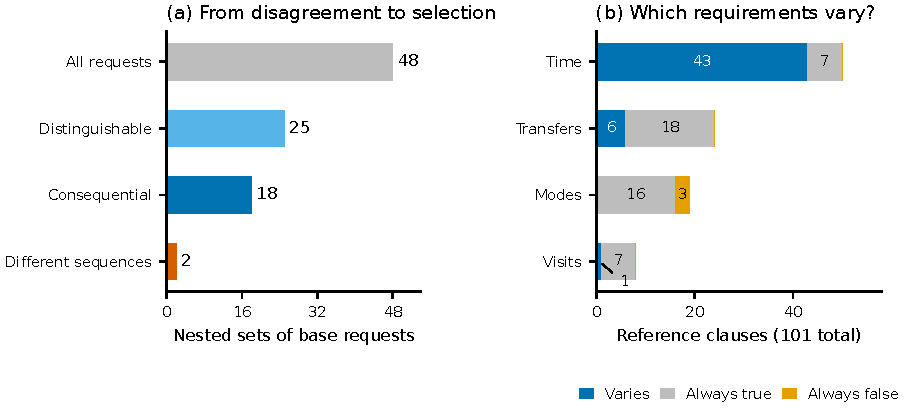
\includegraphics[width=\dimexpr\textwidth-7pt\relax]{diff-original-figures/selector-opportunity.pdf}
}\DIFdelendFL \DIFaddbeginFL \DIFaddFL{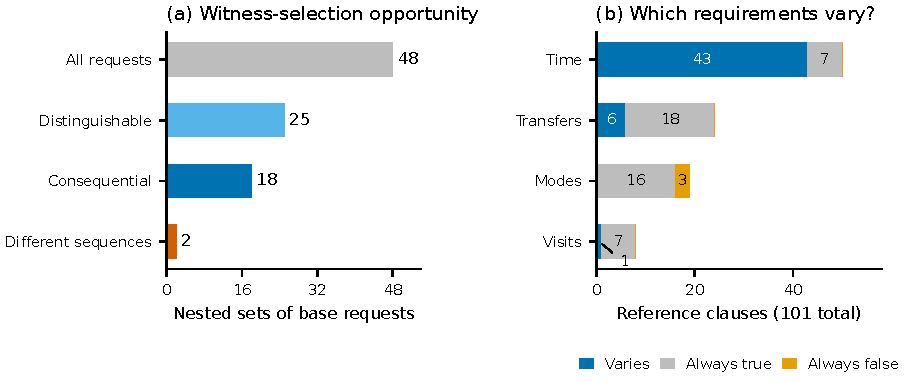
\includegraphics[width=\dimexpr\textwidth-7pt\relax]{figures/selector-opportunity.pdf}
}\DIFaddendFL \caption{\DIFdelbeginFL \DIFdelFL{When does query selection change validation behavior? }\DIFdelendFL Study 1\DIFdelbeginFL \DIFdelFL{connects }\DIFdelendFL \DIFaddbeginFL \DIFaddFL{: witness-selection opportunity and clause tests. Only two of }\DIFaddendFL 48 requests \DIFdelbeginFL \DIFdelFL{to two divergent }\DIFdelendFL \DIFaddbeginFL \DIFaddFL{yield different validation }\DIFaddendFL sequences\DIFdelbeginFL \DIFdelFL{through distinguishable and consequential bundles}\DIFdelendFL . Uniform \DIFaddbeginFL \DIFaddFL{pair }\DIFaddendFL weights and \DIFaddbeginFL \DIFaddFL{shared }\DIFaddendFL tie-breaking explain \DIFaddbeginFL \DIFaddFL{most }\DIFaddendFL identical choices. \DIFdelbeginFL \DIFdelFL{The coverage panel shows variation among }\DIFdelendFL \DIFaddbeginFL \DIFaddFL{Of }\DIFaddendFL 101 \DIFaddbeginFL \DIFaddFL{reference }\DIFaddendFL clauses\DIFaddbeginFL \DIFaddFL{, 51 are constant}\DIFaddendFL ; \DIFdelbeginFL \DIFdelFL{no visit clause tests }\DIFdelendFL \DIFaddbeginFL \DIFaddFL{visits never test }\DIFaddendFL order \DIFdelbeginFL \DIFdelFL{beyond }\DIFdelendFL \DIFaddbeginFL \DIFaddFL{independently of }\DIFaddendFL stop presence.\DIFdelbeginFL \DIFdelFL{These measurements separate algorithmic opportunity from semantic coverage in the bus only setting.}\DIFdelendFL }
\label{fig:opportunity}
\end{figure*}

Both selectors resolve 31/48 requests at budget zero and 33/48 at budgets 1, 2, and 4\DIFdelbegin \DIFdel{, }\DIFdelend \DIFaddbegin \DIFadd{: }\DIFaddend three recoveries and one deterioration, a net 4.17-point gain. \DIFdelbegin \DIFdel{The linked records distinguish this benefit of generic validation from the absence of a }\DIFdelend \DIFaddbegin \DIFadd{This is a validation gain, with no }\DIFaddend weighting advantage. In the deteriorated case, a correct negative judgment removes a wrong formalization whose initial plan was valid, exposing a dependency between candidate \DIFdelbegin \DIFdel{availability }\DIFdelend \DIFaddbegin \DIFadd{coverage }\DIFaddend and preservation of a successful decision.
Each selector returns 30/40 valid feasible plans, five invalid plans, and five false infeasibility conclusions. It identifies 3/8 infeasible requests; five give invalid interpretation outputs. No unresolved or infrastructure failures occur. Budget two adds four judgments per method but changes no plan; budget four adds no judgments. \DIFdelbegin \DIFdel{These stopping records explain the flat accuracy curve through exhausted distinctions}\DIFdelend \DIFaddbegin \DIFadd{No further separating witnesses remain}\DIFaddend . Oracle-witness replay reaches 35/48 for both selectors, identifying a shared opportunity in validation rather than an advantage of weighting.
\DIFdelbegin \DIFdel{Coverage }\DIFdelend \DIFaddbegin \DIFadd{Clause }\DIFaddend checks identify which requirements the benchmark exercises. Of 101 reference clauses, 50 vary, 48 are always satisfied, and three always violated. Six of 24 transfer clauses vary although 45/48 pools offer zero and one transfer journeys\DIFdelbegin \DIFdel{, the two ride bound makes a most one transfer }\DIFdelend \DIFaddbegin \DIFadd{; the two-ride bound makes an at-most-one-transfer }\DIFaddend clause vacuous. All 19 mode clauses are constant, and visits never distinguish ordering beyond stop presence. Removing enumeration caps increases memberships to 77,871 without adding candidate classes or witness partitions for the saved bundles. 
\DIFdelbegin \DIFdel{These measurements direct benchmark development toward meaningful semantic contrasts, rather than simply larger pools.
}\DIFdelend 



\subsection{\DIFdelbegin \DIFdel{Separating Acquisition from Selection}\DIFdelend \DIFaddbegin \DIFadd{Candidate Coverage and Final Decisions}\DIFaddend }

In Study 2, diversified sampling reaches 31/32 \DIFdelbegin \DIFdel{bounded }\DIFdelend candidate coverage compared with 27/32 for independent sampling, while both produce 28/32 correct final outcomes. Figure~\ref{fig:cost} separates \DIFdelbegin \DIFdel{acquisition and decision trajectories }\DIFdelend \DIFaddbegin \DIFadd{candidate coverage and final correctness }\DIFaddend against consumed tokens. All arms begin at 25/32 \DIFaddbegin \DIFadd{candidate }\DIFaddend coverage and correctness\DIFdelbegin \DIFdel{, solver-guided }\DIFdelend \DIFaddbegin \DIFadd{. Solver-guided }\DIFaddend sampling stays there through eight attempts, adding no matching behavior after the shared samples. Mean distinct signatures are 1.41, 1.59, and 1.19 for independent, diversified, and solver-guided sampling. 
\DIFdelbegin \DIFdel{Measuring both trajectories establishes a gain in candidate acquisition and motivates examination of downstream selection.
}\DIFdelend 

\begin{figure*}[t]
\centering
\DIFdelbeginFL \DIFdelFL{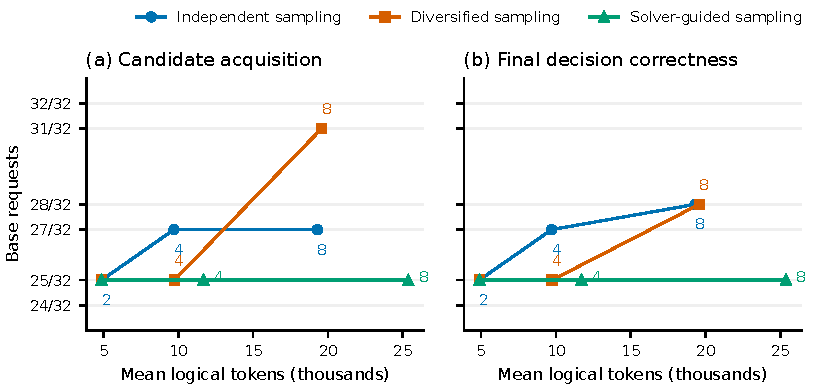
\includegraphics[width=\dimexpr\textwidth-7pt\relax]{diff-original-figures/cost-outcomes.pdf}
}\DIFdelendFL \DIFaddbeginFL \DIFaddFL{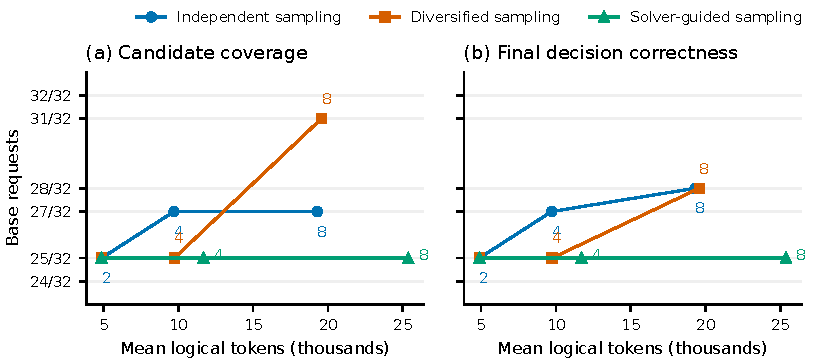
\includegraphics[width=\dimexpr\textwidth-7pt\relax]{figures/cost-outcomes.pdf}
}\DIFaddendFL \caption{\DIFdelbeginFL \DIFdelFL{Where do sampling strategies differ in coverage and cost? }\DIFdelendFL Study 2\DIFdelbeginFL \DIFdelFL{separates matching }\DIFdelendFL \DIFaddbeginFL \DIFaddFL{: }\DIFaddendFL candidate \DIFdelbeginFL \DIFdelFL{availability from }\DIFdelendFL \DIFaddbeginFL \DIFaddFL{coverage and }\DIFaddendFL final correctness \DIFdelbeginFL \DIFdelFL{over 32 requests}\DIFdelendFL \DIFaddbeginFL \DIFaddFL{versus mean logical input plus output tokens}\DIFaddendFL . Labels mark 2, \DIFdelbeginFL \DIFdelFL{2}\DIFdelendFL \DIFaddbeginFL \DIFaddFL{4}\DIFaddendFL , and 8 \DIFdelbeginFL \DIFdelFL{attempt checkpoints, }\DIFdelendFL \DIFaddbeginFL \DIFaddFL{attempts; }\DIFaddendFL lines connect \DIFdelbeginFL \DIFdelFL{only observations}\DIFdelendFL \DIFaddbeginFL \DIFaddFL{observed checkpoints}\DIFaddendFL . \DIFdelbeginFL \DIFdelFL{Cost is mean logical input plus output tokens for generation }\DIFdelendFL \DIFaddbeginFL \DIFaddFL{Generation }\DIFaddendFL and \DIFdelbeginFL \DIFdelFL{prefix }\DIFdelendFL \DIFaddbeginFL \DIFaddFL{checkpoint }\DIFaddendFL validation \DIFaddbeginFL \DIFaddFL{are charged}\DIFaddendFL . \DIFdelbeginFL \DIFdelFL{Diversification increases coverage without changing aggregate final accuracy. Initial }\DIFdelendFL \DIFaddbeginFL \DIFaddFL{The first two }\DIFaddendFL samples are shared\DIFdelbeginFL \DIFdelFL{, allowances remain unexhausted. Paired uncertainty appears in the text}\DIFdelendFL \DIFaddbeginFL \DIFaddFL{; no token allowance is exhausted}\DIFaddendFL .}
\label{fig:cost}
\end{figure*}

\DIFdelbegin \DIFdel{Request level }\DIFdelend \DIFaddbegin \DIFadd{Request-level }\DIFaddend pairing reveals a \DIFdelbegin \DIFdel{further }\DIFdelend distinction behind equal totals\DIFdelbegin \DIFdel{, }\DIFdelend \DIFaddbegin \DIFadd{: }\DIFaddend independent sampling wins on one request, loses on one, and ties on 30 against diversified sampling. Solver guided sampling has zero wins, three losses, and 29 ties against each baseline, with different losing sets. Its correctness difference is $-9.38$ percentage points in each comparison. A 10,000 draw base-request bootstrap gives a descriptive 95\% interval of $[-21.88,0]$ points\DIFaddbegin \DIFadd{; }\DIFaddend independent minus diversified gives $[-9.38,9.38]$. 
\DIFdelbegin \DIFdel{Pairing identifies which decisions change while preserving uncertainty about these small, route dependent samples.
}\DIFdelend The baselines return 24/28 valid feasible plans\DIFdelbegin \DIFdel{, }\DIFdelend \DIFaddbegin \DIFadd{; }\DIFaddend solver-guided sampling returns 21/28. All identify four infeasible requests correctly\DIFdelbegin \DIFdel{, }\DIFdelend \DIFaddbegin \DIFadd{; }\DIFaddend remaining outputs are invalid plans. No final output is unresolved, malformed, or an infrastructure failure; two malformed candidate attempts remain charged. \DIFdelbegin \DIFdel{Solver-guided sampling misses the frozen }\DIFdelend \DIFaddbegin \DIFadd{Before fresh outputs on 13 September 2026, the protocol fixed }\DIFaddend continuation thresholds of \DIFdelbegin \DIFdel{ten points more }\DIFdelend \DIFaddbegin \DIFadd{at least ten percentage points more candidate }\DIFaddend coverage and five points more \DIFdelbegin \DIFdel{correctness over both baselines}\DIFdelend \DIFaddbegin \DIFadd{final correctness than each baseline. Solver-guided sampling met neither threshold}\DIFaddend .



\subsection{Locating Candidate-to-Decision Transitions}

\begin{figure}[t]
\centering
\DIFdelbeginFL \DIFdelFL{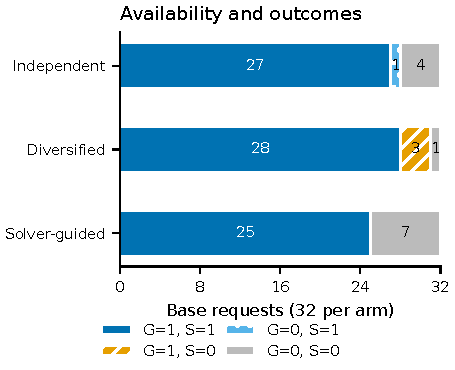
\includegraphics[width=\dimexpr\columnwidth-7pt\relax]{diff-original-figures/joint-outcomes.pdf}
}\DIFdelendFL \DIFaddbeginFL \DIFaddFL{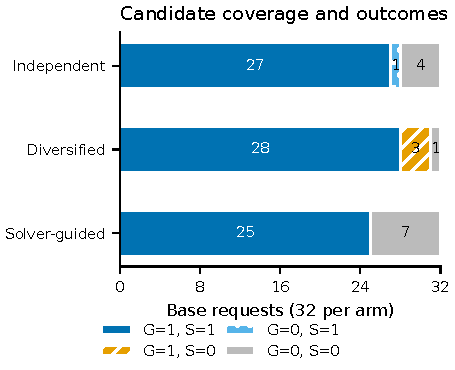
\includegraphics[width=\dimexpr\columnwidth-7pt\relax]{figures/joint-outcomes.pdf}
}\DIFaddendFL \caption{\DIFdelbeginFL \DIFdelFL{How does }\DIFdelendFL \DIFaddbeginFL \DIFaddFL{Joint }\DIFaddendFL candidate \DIFdelbeginFL \DIFdelFL{availability relate to final outcomes? At 8 attempts, each Study 2 arm contains 32 requests. }\DIFdelendFL \DIFaddbeginFL \DIFaddFL{coverage }\DIFaddendFL $G$ \DIFdelbeginFL \DIFdelFL{denotes bounded reference matching availability }\DIFdelendFL and \DIFdelbeginFL \DIFdelFL{$S$ }\DIFdelendFL final correctness \DIFaddbeginFL \DIFaddFL{$S$ at eight attempts (32 requests per arm)}\DIFaddendFL . \DIFdelbeginFL \DIFdelFL{The off diagonal }\DIFdelendFL \DIFaddbeginFL \DIFaddFL{Off-diagonal }\DIFaddendFL cells \DIFdelbeginFL \DIFdelFL{identify }\DIFdelendFL \DIFaddbeginFL \DIFaddFL{show }\DIFaddendFL three \DIFdelbeginFL \DIFdelFL{diversified sampling selection }\DIFdelendFL \DIFaddbeginFL \DIFaddFL{diversified-sampling }\DIFaddendFL losses \DIFaddbeginFL \DIFaddFL{despite a match }\DIFaddendFL and one \DIFdelbeginFL \DIFdelFL{independent sampling }\DIFdelendFL \DIFaddbeginFL \DIFaddFL{independent-sampling }\DIFaddendFL success without a \DIFdelbeginFL \DIFdelFL{matching formalization}\DIFdelendFL \DIFaddbeginFL \DIFaddFL{match}\DIFaddendFL . \DIFdelbeginFL \DIFdelFL{These joint request level }\DIFdelendFL \DIFaddbeginFL \DIFaddFL{All }\DIFaddendFL counts \DIFdelbeginFL \DIFdelFL{distinguish acquisition from }\DIFdelendFL use \DIFdelbeginFL \DIFdelFL{of candidates, references remain }\DIFdelendFL provisional \DIFaddbeginFL \DIFaddFL{references}\DIFaddendFL .}
\label{fig:joint}
\end{figure}

Figure~\ref{fig:joint} shows how candidate \DIFdelbegin \DIFdel{availability }\DIFdelend \DIFaddbegin \DIFadd{coverage }\DIFaddend relates to final outcomes. In $(1,1),(1,0),(0,1),(0,0)$ order the final counts are $(27,0,1,4)$ for independent, $(28,3,0,1)$ for diversified, and $(25,0,0,7)$ for solver-guided sampling. At four attempts, diversification has $(24,1,1,6)$ as equal marginal coverage and correctness of 25 conceal both off-diagonal outcomes. 
\DIFdelbegin \DIFdel{The joint analysis makes acquisition and selection separate development targets instead of treating a common total as a common explanation.
Trace inspection identifies incorrect }\DIFdelend \DIFaddbegin \DIFadd{Relative to the provisional references, trace inspection identifies disagreeing }\DIFaddend judgments eliminating the match in all three diversified final $(1,0)$ cases, 2 false positives and one false negative. A fourth loss appears at four attempts. Each final case ends with one class, so an unresolved tie or unused validation opportunity is not the immediate cause. \DIFdelbegin \DIFdel{Truthful }\DIFdelend \DIFaddbegin \DIFadd{Reference }\DIFaddend labels recover all three \DIFaddbegin \DIFadd{under the same evaluation}\DIFaddend . Across selected witnesses, 11/19 distinct Study 2 judgments and 7/31 Study 1 judgments disagree with provisional references\DIFdelbegin \DIFdel{that these }\DIFdelend \DIFaddbegin \DIFadd{. These cases were not independently adjudicated and }\DIFaddend are not general judge accuracy estimates. 
\DIFdelbegin \DIFdel{Figure~\ref{fig:worked} illustrates how tracing judgments and plans identifies both a lost matching interpretation and a correct decision without one.
}\DIFdelend 

\begin{figure*}[t]
\centering
\DIFdelbeginFL \DIFdelFL{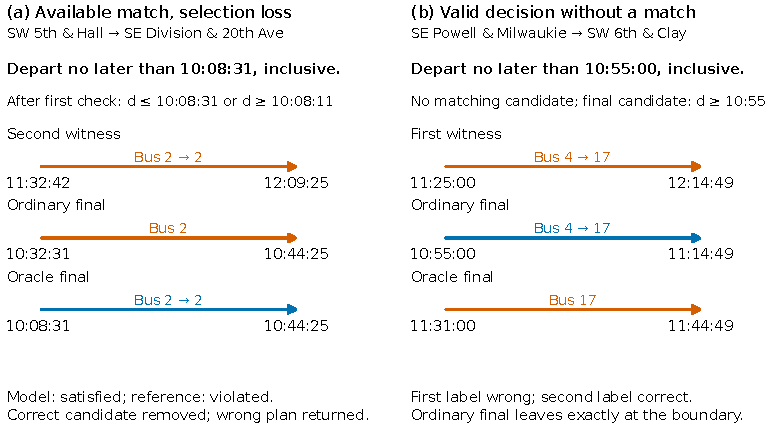
\includegraphics[width=\dimexpr\textwidth-7pt\relax]{diff-original-figures/worked-transit.pdf}
}\DIFdelendFL \DIFaddbeginFL \DIFaddFL{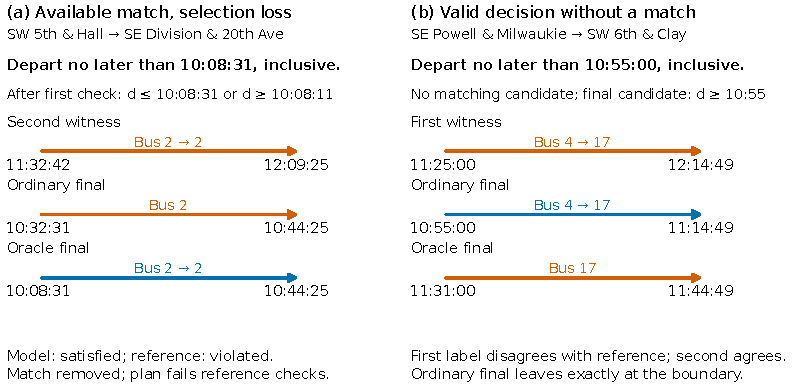
\includegraphics[width=\dimexpr\textwidth-7pt\relax]{figures/worked-transit.pdf}
}\DIFaddendFL \caption{\DIFdelbeginFL \DIFdelFL{Separating interpretation from decision correctness in }\DIFdelendFL Study \DIFdelbeginFL \DIFdelFL{2. The first diversified $(G=1,S=0)$ case at eight attempts }\DIFdelendFL \DIFaddbeginFL \DIFaddFL{2 examples: losing a matching candidate }\DIFaddendFL (left) \DIFdelbeginFL \DIFdelFL{shows a false positive discarding the matching upper bound. The sole independent $(G=0,S=1)$ case there }\DIFdelendFL \DIFaddbeginFL \DIFaddFL{and succeeding without one }\DIFaddendFL (right)\DIFdelbeginFL \DIFdelFL{shows a lower-bound formalization producing a departure exactly at the requested upper bound, truthful first witness rejection takes another path}\DIFdelendFL \DIFaddbeginFL \DIFaddFL{. ``Oracle'' uses reference labels. Correctness is relative to provisional references}\DIFaddendFL . Times are \DIFdelbeginFL \DIFdelFL{scheduled }\DIFdelendFL local \DIFdelbeginFL \DIFdelFL{service }\DIFdelendFL \DIFaddbeginFL \DIFaddFL{scheduled }\DIFaddendFL times on 14 September 2026\DIFaddbeginFL \DIFaddFL{; }\DIFaddendFL arrows \DIFdelbeginFL \DIFdelFL{mark }\DIFdelendFL \DIFaddbeginFL \DIFaddFL{show }\DIFaddendFL endpoints, not a scaled time axis.\DIFdelbeginFL \DIFdelFL{These illustrative cases explain distinct joint cells, not their population prevalence.}\DIFdelendFL }
\label{fig:worked}
\end{figure*}

The left example requests departure by 10:08:31. A correct first judgment leaves the matching upper bound and a wrong lower bound. Accepting a second witness departing at 11:32:42 removes the match and yields a 10:32:31 plan. \DIFdelbegin \DIFdel{Truthful }\DIFdelend \DIFaddbegin \DIFadd{Reference-label }\DIFaddend replay returns a valid 10:08:31 departure. 
\DIFdelbegin \DIFdel{This trace identifies a specific judgment check to investigate, without attributing every selection loss to the same cause.
}\DIFdelend 

\subsection{Distinguishing Oracle Measurements}

Oracle witness replay substitutes reference labels while retaining bounded elimination and the first surviving candidate. Correctness is 27/32, 31/32, and 25/32: equal to coverage totals here, but measuring a different procedure.
Figure~\ref{fig:worked} (right) explains independent sampling's 28 ordinary versus 27 oracle witness successes. The request requires departure by 10:55\DIFdelbegin \DIFdel{, }\DIFdelend \DIFaddbegin \DIFadd{; }\DIFaddend no candidate matches throughout the pool. A wrong positive on an 11:25 departure removes one candidate. A correct second positive retains a lower-bound candidate, whose optimal plan leaves exactly at 10:55 and satisfies the request. \DIFdelbegin \DIFdel{Truthful }\DIFdelend \DIFaddbegin \DIFadd{Reference-label }\DIFaddend first witness rejection instead retains a candidate producing an 11:31 departure. Thus \DIFdelbegin \DIFdel{truthful }\DIFdelend \DIFaddbegin \DIFadd{reference }\DIFaddend labels can change the elimination path and lose a valid decision: this procedure is not an accuracy ceiling.
A separate diagnostic asks whether \emph{any existing candidate's \DIFdelbegin \DIFdel{deterministically }\DIFdelend selected output} is correct\DIFdelbegin \DIFdel{,  }\DIFdelend \DIFaddbegin \DIFadd{: }\DIFaddend 28/32, 31/32, and 25/32 at eight attempts. This \DIFdelbegin \DIFdel{restricted best of candidate outputs measure is neither an ordinary selector nor an unrestricted planning bound. Distinguishing it from }\DIFdelend \DIFaddbegin \DIFadd{best-of-candidate-outputs measure is restricted to existing plans; it differs from both }\DIFaddend $G$ and \DIFdelbegin \DIFdel{oracle-witness correctness avoids interpreting ordinary success as exceeding an oracle ceiling}\DIFdelend \DIFaddbegin \DIFadd{reference-label replay}\DIFaddend .

\subsection{Relating Inference Cost to Discovery}

Final prefix logical input/output tokens total 617,643, 626,497, and 811,760 for independent, diversified, and solver-guided sampling across 32 requests each. Solver guided overhead is 31.43\% and 29.57\%, relative to the corresponding baseline's consumed generation plus validation total. Logical calls are 266, 269, and 262. \DIFdelbegin \DIFdel{Together with the discovery curves, these measurements locate additional expenditure without }\DIFdelend \DIFaddbegin \DIFadd{The extra tokens produced no }\DIFaddend additional matching candidates\DIFdelbegin \DIFdel{in this feedback variant; equal allowances or fewer calls alone would not expose that tradeoff.
Across prefixes, counting generation once per trajectory and each prefix's judgments gives }\DIFdelend \DIFaddbegin \DIFadd{.
Across checkpoints, generation is counted once per sampling sequence and judgments once per checkpoint: }\DIFaddend 833 logical calls and 2,081,931 tokens. \DIFdelbegin \DIFdel{Exact caching }\DIFdelend \DIFaddbegin \DIFadd{Caching }\DIFaddend reduces actual fresh compute to 659 calls and 1,743,059 tokens. \DIFdelbegin \DIFdel{Sampling used 1,207.31 measured GPU-resident seconds plus 53.37 for development and a conservative 60-second allowance. The selector study used 358 calls and 681.62 seconds plus 30 seconds}\DIFdelend \DIFaddbegin \DIFadd{The companion records GPU times and development costs}\DIFaddend . Shared outputs retain full per-arm logical charges.



\section{\uppercase{Applying the Framework}}
\label{sec:recommendations}

\noindent For each \DIFdelbegin \DIFdel{base }\DIFdelend request, retain \DIFdelbegin \DIFdel{the universe, source requirements, separate references, raw }\DIFdelend \DIFaddbegin \DIFadd{its pool, reference rules, generated }\DIFaddend candidates, signatures, \DIFaddbegin \DIFadd{selected }\DIFaddend plans, witnesses, judgments, \DIFdelbegin \DIFdel{updates, and cost. Joint }\DIFdelend \DIFaddbegin \DIFadd{and costs. Report joint }\DIFaddend $(G,S)$ cells and \DIFdelbegin \DIFdel{separate output categoriesthen connect aggregate differences to the intermediate behaviors producing them.
This reusable procedure supports three recommendations.
Construct informative tasks, which  checks clause variation and conditional relevance before model evaluation. Identify journeys exposing intended distinctions: different }\DIFdelend \DIFaddbegin \DIFadd{output categories, then inspect the traces behind them.
First, test clauses before evaluating models: include journeys on both sides of a time or transfer limit, and different visit }\DIFaddend orders with the same stops\DIFdelbegin \DIFdel{, transfers around a limit, or departures around a boundary. Pool size alone cannot certify coverage across experiments.
Contrast based inclusion rules improve informativeness without selecting cases for a preferred method. Target components using evidence for diversification's increased coverage and three traced selection losses motivate investigating validation before adding candidates. Conversely, check candidate selected plans in $(0,0)$ cases before attributing failure to missing alternatives. The }\DIFdelend \DIFaddbegin \DIFadd{. Larger pools alone do not ensure useful contrasts.
Second, use the joint cells to choose what to inspect. Diversification increased candidate coverage without increasing final correctness. The three traced losses point to validation as a component to investigate, conditional on the references. Independent review of those references and disputed judgments should precede a claim about judge error. A }\DIFaddend $(0,1)$ \DIFdelbegin \DIFdel{cell }\DIFdelend \DIFaddbegin \DIFadd{outcome }\DIFaddend preserves a correct plan's value without certifying its formalization.
\DIFdelbegin \DIFdel{Precise oracle interventions clarify the remaining opportunity, truthful witness selection tests an altered validation path, whereas best-of-candidate outputs measures available decisions.
Connect cost to observable change, toreport }\DIFdelend \DIFaddbegin \DIFadd{Third, report }\DIFaddend tokens, logical \DIFdelbegin \DIFdel{charges}\DIFdelend \DIFaddbegin \DIFadd{calls}\DIFaddend , caching, and stopping reasons alongside \DIFdelbegin \DIFdel{attempt budgets. These distinguish feedback expenditure without new matches , unused allowances, and checks leaving plansunchanged. Shared time normalization remains a useful engineering baseline. Freeze resource rules and assess component changes on fresh data.
Aggregate accuracy remains valuable, and a component gain can precede an accuracy gain}\DIFdelend \DIFaddbegin \DIFadd{sample allowances. Here they reveal feedback costs without additional matches and extra judgments without changed plans}\DIFaddend .
The framework \DIFdelbegin \DIFdel{helps interpret both. Although the tested weighting and feedback variants do not justify expansion, their analysis identifies measurement requirements and component targets. Applying the framework }\DIFdelend \DIFaddbegin \DIFadd{supplies diagnostic information; it }\DIFaddend has not itself been shown to improve accuracy or reduce cost. \DIFaddbegin \DIFadd{The results do not support expanding the tested weighting or feedback variants.
}\DIFaddend 


\section{\uppercase{Limitations}}
\label{sec:limitations}


\noindent The studies contain 48 and 32 \DIFdelbegin \DIFdel{bases}\DIFdelend \DIFaddbegin \DIFadd{requests}\DIFaddend , one model, and one replicate. Constructed wording, overlapping services, and a shared translation/judgment model \DIFdelbegin \DIFdel{constrain generalization. Selection and normalization differ across studies; accuracies must not be pooled}\DIFdelend \DIFaddbegin \DIFadd{limit generalization. Different protocols prevent pooling the studies}\DIFaddend . Bootstrap intervals exclude annotation uncertainty, route dependence, and variation over models and prompts.
\DIFdelbegin \DIFdel{Separate reference code reduces implementation dependence; developer checks do not establish independent annotation validity}\DIFdelend \DIFaddbegin \DIFadd{References remain provisional: the 80-request worksheet has no completed human-review decisions}\DIFaddend . Systematic wording errors could affect $G$ and $S$ together\DIFdelbegin \DIFdel{. No clear correction was found in the selector audit. A worksheet awaits actual author or collaborator review.
The universe is }\DIFdelend \DIFaddbegin \DIFadd{, so disputed judgments require independent review.
All claims concern bounded pools, }\DIFaddend not the full network. \DIFdelbegin \DIFdel{Conditional infeasibility is weaker than real-world impossibility. The subset excludes available non-bus services; transfer }\DIFdelend \DIFaddbegin \DIFadd{Non-bus services, midnight, and daylight saving are untested. Transfer }\DIFaddend clauses can be vacuous \DIFdelbegin \DIFdel{, visit clauses }\DIFdelend \DIFaddbegin \DIFadd{and visits }\DIFaddend do not independently test order\DIFdelbegin \DIFdel{, and daytime requests do not test midnight or daylight saving}\DIFdelend . Study 2 \DIFdelbegin \DIFdel{'s stronger clause checks improve informativeness without broadening these claims}\DIFdelend \DIFaddbegin \DIFadd{improves clause tests without resolving these limits}\DIFaddend . Matching signatures can \DIFdelbegin \DIFdel{conceal semantic differences lacking counterexamples. Clause level signatures expose variation masked by a rejecting conjunct, but source clause associations are not always available. This framework therefore measures bounded behavior, not unrestricted source fidelity  selected witness disagreements are not general judge error rates.
A stronger or independently trained judge, different prompts, or broader coverage }\DIFdelend \DIFaddbegin \DIFadd{hide differences for which the pool lacks examples; clause associations with source wording may also be unavailable.
Stronger judges, other prompts, and broader pools }\DIFaddend could change the comparisons. Repeated lower-bound readings do not establish feedback anchoring. This \DIFdelbegin \DIFdel{position developed through }\DIFdelend \DIFaddbegin \DIFadd{framework developed from }\DIFaddend exploratory studies, not \DIFdelbegin \DIFdel{as }\DIFdelend a preregistered reporting hypothesis\DIFdelbegin \DIFdel{. Its demonstrated value is the diagnostic information obtained here applicability }\DIFdelend \DIFaddbegin \DIFadd{; its value }\DIFaddend across models and domains remains \DIFdelbegin \DIFdel{open}\DIFdelend \DIFaddbegin \DIFadd{untested}\DIFaddend .


\section{\uppercase{Conclusion}}
\label{sec:conclusion}

\noindent \DIFdelbegin \DIFdel{We propose a framework linking tested constraints, available interpretations, validation behavior, decisions, and cost. The transit studies demonstrate its explanatory value that opportunity analysis characterizes when selectors can act differently, and joint outcomes separate candidate acquisition from decision selection. The reproducible procedure makes these distinctions available to other planning evaluations. Future studies should measure both available interpretations and selected decisions, stating semantic coverage and resource use explicitly. These connections support targeted development and clearer interpretation of progress beyond aggregate accuracy}\DIFdelend \DIFaddbegin \DIFadd{Reporting candidate coverage and final correctness jointly explains differences hidden by aggregate accuracy. Clause tests show what the benchmark exercises, while validation traces and costs show how available candidates are used. In these studies, weighting rarely changed witness choices, and greater candidate coverage did not guarantee better final decisions. Next, disputed reference cases need independent review, followed by tests with other models and more varied pools. These steps would test whether the same diagnosis remains useful beyond this setting.
}


\subsection*{\DIFadd{Code and Data Availability}}
\label{sec:availability}
\DIFadd{Code, prompts, constructed requests, provisional references, frozen protocols, and compact results are available in the }\href{https://github.com/mantzaris/LLMplanningContraintsDecision}{project repository}\DIFadd{. The companion }\texttt{\DIFadd{reproducibility.pdf}} \DIFadd{documents exact templates and commands. The frozen feed and full raw generation logs remain in project storage, outside the public repository; full historical replay requires those files. Compact tables and figures can be inspected without them}\DIFaddend .

\subsection*{AI Assistance Disclosure}
\label{sec:ai}
OpenAI Codex \cite{codex} assisted with the code and environment setup.


\begin{thebibliography}{99}
\bibitem[Amonkar et~al., 2026]{amonkar}
Amonkar, R., Kayan, C.~E., Lai, Q., Le~Bras, R., and Zhang, L. (2026).
A reality check of language models as formalizers on constraint satisfaction problems.
\emph{arXiv:2505.13252v6}. Preprint; first submitted 2025.
\href{https://arxiv.org/abs/2505.13252v6}{doi:10.48550/arXiv.2505.13252}.

\bibitem[GTFS, 2026]{gtfs}
GTFS (2026). Schedule reference.
\url{https://gtfs.org/documentation/schedule/reference/}. Accessed 13 September 2026.

\bibitem[Mendoza et~al., 2026]{artemis}
Mendoza, D., Mavridou, A., Katis, A., and Trippel, C. (2026).
Automating requirements formalization: Using LLMs and low-complexity distinguishing traces for semantic validation.
In \emph{48th IEEE/ACM International Conference on Software Engineering (ICSE)}.
\href{https://doi.org/10.1145/3744916.3787815}{doi:10.1145/3744916.3787815}.

\bibitem[OpenAI, 2026]{codex}
OpenAI (2026). Codex. AI assistance tool.
\url{https://openai.com/codex/}. Accessed 13 September 2026.

\bibitem[Qwen Team, 2024]{qwen}
Qwen Team (2024). Qwen2.5-7B-Instruct: Official model card.
\url{https://huggingface.co/Qwen/Qwen2.5-7B-Instruct}. Accessed 13 September 2026.

\bibitem[Raza and Milic-Frayling, 2025]{ssv}
Raza, M. and Milic-Frayling, N. (2025).
Instantiation-based formalization of logical reasoning tasks using language models and logical solvers.
In \emph{Proceedings of IJCAI-25}, pages 4633--4641.
\href{https://doi.org/10.24963/ijcai.2025/516}{doi:10.24963/ijcai.2025/516}.

\bibitem[Singh et~al., 2026]{verge}
Singh, V., Cassel, D., Weir, N., Feng, N., and Bayless, S. (2026).
VERGE: Formal refinement and guidance engine for verifiable LLM reasoning.
\emph{arXiv:2601.20055v2}. Preprint.
\href{https://arxiv.org/abs/2601.20055v2}{doi:10.48550/arXiv.2601.20055}\DIFaddbegin \DIFadd{.
}

\bibitem[Tantakoun et~al., 2025]{tantakoun}
\DIFadd{Tantakoun, M., Muise, C., and Zhu, X. (2025).
LLMs as planning formalizers: A survey for leveraging large language models to construct automated planning models.
In }\emph{\DIFadd{Findings of the Association for Computational Linguistics: ACL 2025}}\DIFadd{, pages 25167--25188.
}\href{https://doi.org/10.18653/v1/2025.findings-acl.1291}{doi:10.18653/v1/2025.findings-acl.1291}\DIFaddend .

\bibitem[TriMet, 2026]{trimet}
TriMet (2026). GTFS schedule data.
\url{https://developer.trimet.org/GTFS.shtml}. Feed version 20260823-20260910-0900; acquired September 2026.

\bibitem[Wang et~al., 2026]{diversity}
Wang, T., Liu, Z., Chen, Y., Light, J., Liu, W., Chen, H., Zhang, X., and Cheng, W. (2026).
On the effect of sampling diversity in scaling LLM inference.
\emph{arXiv:2502.11027v5}. Preprint; first submitted 2025.
\href{https://arxiv.org/abs/2502.11027v5}{doi:10.48550/arXiv.2502.11027}.
\end{thebibliography}
\end{document}
